
%% bare_conf.tex
%% V1.4b
%% 2015/08/26
%% by Michael Shell
%% See:
%% http://www.michaelshell.org/
%% for current contact information.
%%
%% This is a skeleton file demonstrating the use of IEEEtran.cls
%% (requires IEEEtran.cls version 1.8b or later) with an IEEE
%% conference paper.
%%
%% Support sites:
%% http://www.michaelshell.org/tex/ieeetran/
%% http://www.ctan.org/pkg/ieeetran
%% and
%% http://www.ieee.org/

%%*************************************************************************
%% Legal Notice:
%% This code is offered as-is without any warranty either expressed or
%% implied; without even the implied warranty of MERCHANTABILITY or
%% FITNESS FOR A PARTICULAR PURPOSE! 
%% User assumes all risk.
%% In no event shall the IEEE or any contributor to this code be liable for
%% any damages or losses, including, but not limited to, incidental,
%% consequential, or any other damages, resulting from the use or misuse
%% of any information contained here.
%%
%% All comments are the opinions of their respective authors and are not
%% necessarily endorsed by the IEEE.
%%
%% This work is distributed under the LaTeX Project Public License (LPPL)
%% ( http://www.latex-project.org/ ) version 1.3, and may be freely used,
%% distributed and modified. A copy of the LPPL, version 1.3, is included
%% in the base LaTeX documentation of all distributions of LaTeX released
%% 2003/12/01 or later.
%% Retain all contribution notices and credits.
%% ** Modified files should be clearly indicated as such, including  **
%% ** renaming them and changing author support contact information. **
%%*************************************************************************


% *** Authors should verify (and, if needed, correct) their LaTeX system  ***
% *** with the testflow diagnostic prior to trusting their LaTeX platform ***
% *** with production work. The IEEE's font choices and paper sizes can   ***
% *** trigger bugs that do not appear when using other class files.       ***                          ***
% The testflow support page is at:
% http://www.michaelshell.org/tex/testflow/



\documentclass[conference]{IEEEtran}
\IEEEoverridecommandlockouts
\PassOptionsToPackage{bookmarks={false}}{hyperref}
% Some Computer Society conferences also require the compsoc mode option,
% but others use the standard conference format.
%
% If IEEEtran.cls has not been installed into the LaTeX system files,
% manually specify the path to it like:
% \documentclass[conference]{../sty/IEEEtran}





% Some very useful LaTeX packages include:
% (uncomment the ones you want to load)


% *** MISC UTILITY PACKAGES ***
%
\usepackage{ifpdf}
% Heiko Oberdiek's ifpdf.sty is very useful if you need conditional
% compilation based on whether the output is pdf or dvi.
% usage:
% \ifpdf
%   % pdf code
% \else
%   % dvi code
% \fi
% The latest version of ifpdf.sty can be obtained from:
% http://www.ctan.org/pkg/ifpdf
% Also, note that IEEEtran.cls V1.7 and later provides a builtin
% \ifCLASSINFOpdf conditional that works the same way.
% When switching from latex to pdflatex and vice-versa, the compiler may
% have to be run twice to clear warning/error messages.






% *** CITATION PACKAGES ***
%
\usepackage{cite}
% cite.sty was written by Donald Arseneau
% V1.6 and later of IEEEtran pre-defines the format of the cite.sty package
% \cite{} output to follow that of the IEEE. Loading the cite package will
% result in citation numbers being automatically sorted and properly
% "compressed/ranged". e.g., [1], [9], [2], [7], [5], [6] without using
% cite.sty will become [1], [2], [5]--[7], [9] using cite.sty. cite.sty's
% \cite will automatically add leading space, if needed. Use cite.sty's
% noadjust option (cite.sty V3.8 and later) if you want to turn this off
% such as if a citation ever needs to be enclosed in parenthesis.
% cite.sty is already installed on most LaTeX systems. Be sure and use
% version 5.0 (2009-03-20) and later if using hyperref.sty.
% The latest version can be obtained at:
% http://www.ctan.org/pkg/cite
% The documentation is contained in the cite.sty file itself.
\usepackage{hyperref}





% *** GRAPHICS RELATED PACKAGES ***
%
\ifCLASSINFOpdf
   \usepackage[pdftex]{graphicx}
  % declare the path(s) where your graphic files are
  % \graphicspath{{../pdf/}{../jpeg/}}
  % and their extensions so you won't have to specify these with
  % every instance of \includegraphics
  % \DeclareGraphicsExtensions{.pdf,.jpeg,.png}
\else
  % or other class option (dvipsone, dvipdf, if not using dvips). graphicx
  % will default to the driver specified in the system graphics.cfg if no
  % driver is specified.
  % \usepackage[dvips]{graphicx}
  % declare the path(s) where your graphic files are
  % \graphicspath{{../eps/}}
  % and their extensions so you won't have to specify these with
  % every instance of \includegraphics
  % \DeclareGraphicsExtensions{.eps}
\fi
% graphicx was written by David Carlisle and Sebastian Rahtz. It is
% required if you want graphics, photos, etc. graphicx.sty is already
% installed on most LaTeX systems. The latest version and documentation
% can be obtained at: 
% http://www.ctan.org/pkg/graphicx
% Another good source of documentation is "Using Imported Graphics in
% LaTeX2e" by Keith Reckdahl which can be found at:
% http://www.ctan.org/pkg/epslatex
%
% latex, and pdflatex in dvi mode, support graphics in encapsulated
% postscript (.eps) format. pdflatex in pdf mode supports graphics
% in .pdf, .jpeg, .png and .mps (metapost) formats. Users should ensure
% that all non-photo figures use a vector format (.eps, .pdf, .mps) and
% not a bitmapped formats (.jpeg, .png). The IEEE frowns on bitmapped formats
% which can result in "jaggedy"/blurry rendering of lines and letters as
% well as large increases in file sizes.
%
% You can find documentation about the pdfTeX application at:
% http://www.tug.org/applications/pdftex





% *** MATH PACKAGES ***
%
%\usepackage{amsmath}
% A popular package from the American Mathematical Society that provides
% many useful and powerful commands for dealing with mathematics.
%
% Note that the amsmath package sets \interdisplaylinepenalty to 10000
% thus preventing page breaks from occurring within multiline equations. Use:
%\interdisplaylinepenalty=2500
% after loading amsmath to restore such page breaks as IEEEtran.cls normally
% does. amsmath.sty is already installed on most LaTeX systems. The latest
% version and documentation can be obtained at:
% http://www.ctan.org/pkg/amsmath





% *** SPECIALIZED LIST PACKAGES ***
%
%\usepackage{algorithmic}
% algorithmic.sty was written by Peter Williams and Rogerio Brito.
% This package provides an algorithmic environment fo describing algorithms.
% You can use the algorithmic environment in-text or within a figure
% environment to provide for a floating algorithm. Do NOT use the algorithm
% floating environment provided by algorithm.sty (by the same authors) or
% algorithm2e.sty (by Christophe Fiorio) as the IEEE does not use dedicated
% algorithm float types and packages that provide these will not provide
% correct IEEE style captions. The latest version and documentation of
% algorithmic.sty can be obtained at:
% http://www.ctan.org/pkg/algorithms
% Also of interest may be the (relatively newer and more customizable)
% algorithmicx.sty package by Szasz Janos:
% http://www.ctan.org/pkg/algorithmicx




% *** ALIGNMENT PACKAGES ***
%
%\usepackage{array}
% Frank Mittelbach's and David Carlisle's array.sty patches and improves
% the standard LaTeX2e array and tabular environments to provide better
% appearance and additional user controls. As the default LaTeX2e table
% generation code is lacking to the point of almost being broken with
% respect to the quality of the end results, all users are strongly
% advised to use an enhanced (at the very least that provided by array.sty)
% set of table tools. array.sty is already installed on most systems. The
% latest version and documentation can be obtained at:
% http://www.ctan.org/pkg/array


% IEEEtran contains the IEEEeqnarray family of commands that can be used to
% generate multiline equations as well as matrices, tables, etc., of high
% quality.



\usepackage{subfigure}
\usepackage{graphicx}
\usepackage{multirow}
\usepackage{geometry}
\usepackage{amsmath}
\usepackage{amssymb}
\usepackage{amsthm}
\theoremstyle{definition}
\newtheorem{definition}{Definition}[section]

% *** SUBFIGURE PACKAGES ***
%\ifCLASSOPTIONcompsoc
%  \usepackage[caption=false,font=normalsize,labelfont=sf,textfont=sf]{subfig}
%\else
%  \usepackage[caption=false,font=footnotesize]{subfig}
%\fi
% subfig.sty, written by Steven Douglas Cochran, is the modern replacement
% for subfigure.sty, the latter of which is no longer maintained and is
% incompatible with some LaTeX packages including fixltx2e. However,
% subfig.sty requires and automatically loads Axel Sommerfeldt's caption.sty
% which will override IEEEtran.cls' handling of captions and this will result
% in non-IEEE style figure/table captions. To prevent this problem, be sure
% and invoke subfig.sty's "caption=false" package option (available since
% subfig.sty version 1.3, 2005/06/28) as this is will preserve IEEEtran.cls
% handling of captions.
% Note that the Computer Society format requires a larger sans serif font
% than the serif footnote size font used in traditional IEEE formatting
% and thus the need to invoke different subfig.sty package options depending
% on whether compsoc mode has been enabled.
%
% The latest version and documentation of subfig.sty can be obtained at:
% http://www.ctan.org/pkg/subfig




% *** FLOAT PACKAGES ***
%
%\usepackage{fixltx2e}
% fixltx2e, the successor to the earlier fix2col.sty, was written by
% Frank Mittelbach and David Carlisle. This package corrects a few problems
% in the LaTeX2e kernel, the most notable of which is that in current
% LaTeX2e releases, the ordering of single and double column floats is not
% guaranteed to be preserved. Thus, an unpatched LaTeX2e can allow a
% single column figure to be placed prior to an earlier double column
% figure.
% Be aware that LaTeX2e kernels dated 2015 and later have fixltx2e.sty's
% corrections already built into the system in which case a warning will
% be issued if an attempt is made to load fixltx2e.sty as it is no longer
% needed.
% The latest version and documentation can be found at:
% http://www.ctan.org/pkg/fixltx2e


%\usepackage{stfloats}
% stfloats.sty was written by Sigitas Tolusis. This package gives LaTeX2e
% the ability to do double column floats at the bottom of the page as well
% as the top. (e.g., "\begin{figure*}[!b]" is not normally possible in
% LaTeX2e). It also provides a command:
%\fnbelowfloat
% to enable the placement of footnotes below bottom floats (the standard
% LaTeX2e kernel puts them above bottom floats). This is an invasive package
% which rewrites many portions of the LaTeX2e float routines. It may not work
% with other packages that modify the LaTeX2e float routines. The latest
% version and documentation can be obtained at:
% http://www.ctan.org/pkg/stfloats
% Do not use the stfloats baselinefloat ability as the IEEE does not allow
% \baselineskip to stretch. Authors submitting work to the IEEE should note
% that the IEEE rarely uses double column equations and that authors should try
% to avoid such use. Do not be tempted to use the cuted.sty or midfloat.sty
% packages (also by Sigitas Tolusis) as the IEEE does not format its papers in
% such ways.
% Do not attempt to use stfloats with fixltx2e as they are incompatible.
% Instead, use Morten Hogholm'a dblfloatfix which combines the features
% of both fixltx2e and stfloats:
%
% \usepackage{dblfloatfix}
% The latest version can be found at:
% http://www.ctan.org/pkg/dblfloatfix




% *** PDF, URL AND HYPERLINK PACKAGES ***
%
%\usepackage{url}
% url.sty was written by Donald Arseneau. It provides better support for
% handling and breaking URLs. url.sty is already installed on most LaTeX
% systems. The latest version and documentation can be obtained at:
% http://www.ctan.org/pkg/url
% Basically, \url{my_url_here}.




% *** Do not adjust lengths that control margins, column widths, etc. ***
% *** Do not use packages that alter fonts (such as pslatex).         ***
% There should be no need to do such things with IEEEtran.cls V1.6 and later.
% (Unless specifically asked to do so by the journal or conference you plan
% to submit to, of course. )


% correct bad hyphenation here
\hyphenation{op-tical net-works semi-conduc-tor}


\begin{document}
%
% paper title
% Titles are generally capitalized except for words such as a, an, and, as,
% at, but, by, for, in, nor, of, on, or, the, to and up, which are usually
% not capitalized unless they are the first or last word of the title.
% Linebreaks \\ can be used within to get better formatting as desired.
% Do not put math or special symbols in the title.
\title{Model Checking FMI Co-simulation Using Timed Automata}


% author names and affiliations
% use a multiple column layout for up to three different
% affiliations
\author{\IEEEauthorblockN{Kaiqiang Jiang, Chunlin Guan, Jiahui Wang, Dehui Du*}
\IEEEauthorblockA{Shanghai Key Laboratory of Trustworthy Computing,\\ East China Normal University, Shanghai, 200062, China\\
Email: dhdu@sei.ecnu.edu.cn}
\thanks{*Corresponding Author}
}

% conference papers do not typically use \thanks and this command
% is locked out in conference mode. If really needed, such as for
% the acknowledgment of grants, issue a \IEEEoverridecommandlockouts
% after \documentclass

% for over three affiliations, or if they all won't fit within the width
% of the page, use this alternative format:
% 
%\author{\IEEEauthorblockN{Michael Shell\IEEEauthorrefmark{1},
%Homer Simpson\IEEEauthorrefmark{2},
%James Kirk\IEEEauthorrefmark{3}, 
%Montgomery Scott\IEEEauthorrefmark{3} and
%Eldon Tyrell\IEEEauthorrefmark{4}}
%\IEEEauthorblockA{\IEEEauthorrefmark{1}School of Electrical and Computer Engineering\\
%Georgia Institute of Technology,
%Atlanta, Georgia 30332--0250\\ Email: see http://www.michaelshell.org/contact.html}
%\IEEEauthorblockA{\IEEEauthorrefmark{2}Twentieth Century Fox, Springfield, USA\\
%Email: homer@thesimpsons.com}
%\IEEEauthorblockA{\IEEEauthorrefmark{3}Starfleet Academy, San Francisco, California 96678-2391\\
%Telephone: (800) 555--1212, Fax: (888) 555--1212}
%\IEEEauthorblockA{\IEEEauthorrefmark{4}Tyrell Inc., 123 Replicant Street, Los Angeles, California 90210--4321}}




% use for special paper notices
%\IEEEspecialpapernotice{(Invited Paper)}




% make the title area
\maketitle

% As a general rule, do not put math, special symbols or citations
% in the abstract
\begin{abstract}
The growing complexity of Cyber-Physical Systems (CPS) increasingly challenges the existing methods and techniques. The correctness of coordination between heterogeneous components of CPS is still a challenging problem. 
%A promising approach for verifying coordination behaviour of CPS is simulation-based verification,
The coordination of CPS could be implemented with co-simulation technology, which uses Functional Mock-up Interface (FMI) techniques to generate simulations of heterogeneous components in CPS. However, the master algorithm for co-simulation may be livelock or deadlock. Moreover, the architecture modeling of CPS may also introduce an algebraic loop which is a feedback loop resulting in cyclic dependencies. To solve these problems, we propose a novel approach for model checking several properties of coordination such as deadlock, liveness and reachability. We model the architecture of CPS with SysML Block Definition Diagrams (BDDs) and Internal Block Diagrams (IBDs), which capture the dependence of Functional Mock-up Units (FMUs) and the orchestration of the master algorithm. According to BDD models, the coordination between components is implemented with the master algorithm. We model three various master algorithms with Timed Automata (TA). Besides, we encode FMU components with TA to bridge the semantics gap between FMU and TA. With the help of the model checker UPPAAL, we can analyse the correctness of the master algorithms and detect whether there is an algebraic loop in the architecture. By this way, the coordination of CPS is verified with model checking.

%This work aims at providing an effective approach to verify the coordination of heterogeneous components in CPS.
To illustrate the feasibility of our approach, the case study water tank is presented. The experiment results show that our approach facilitates model checking coordination of CPS. The novelty of our work is that our approach provides a feasible framework for model checking coordination of CPS with TA. 
\end{abstract}
\begin{IEEEkeywords}
Co-simulation, Master algorithm, Functional Mock-up Interface, Timed automata, Model checking.
\end{IEEEkeywords}
% no keywords




% For peer review papers, you can put extra information on the cover
% page as needed:
% \ifCLASSOPTIONpeerreview
% \begin{center} \bfseries EDICS Category: 3-BBND \end{center}
% \fi
%
% For peerreview papers, this IEEEtran command inserts a page break and
% creates the second title. It will be ignored for other modes.
\IEEEpeerreviewmaketitle



\section{Introduction}

\textit{Cyber-physical systems} (CPS) are integration of computation with physical processes whose behavior is defined by both computational and physical parts of the system \cite{Zanero17}. Embedded computers and networks monitor and control the physical processes, usually with feedback loops where physical processes affect computations and vice versa. The heterogeneity is one of the main characteristics of CPS. The components of CPS are of various types, requiring interfacing and interoperability across multiple platforms and different models of computation. Verifying coordination of heterogeneous CPS is a challenging problem. The coordination between heterogeneous components of CPS could be implemented with Functional Mock-up Interface (FMI) based co-simulation technology. The FMI standard was first developed in the MODELISAR project started in 2008 and supported by a large number of software companies and research centers \cite{ClauMODELISAR}. FMI supports simulation of complex systems composed of heterogeneous components, by coupling different models with their own solvers in a co-simulation environment.

In this paper, we focus on verifying the coordination of CPS which implemented with FMI 2.0 \cite{Cremona2006Automatic} based co-simulation. The key point is Master Algorithm (MA) \cite{AckerDVM15} and connector configuration between Functional Mock-up Units (FMUs) \cite{Tripakis15}, which specifies the orchestration and the exchange of data among FMUs during the whole coordination process. To ensure the correctness of coordination, we need to verify MA and connector configuration with model checking. However, MA is not a part of FMI standard. This implies that the user or tool vendor needs to develop a sophisticated orchestration algorithm for the problem at hand. 
%Is the MA deadlock free?
%Dose the MA satisfy the reachability? To solve these problem, we can verify the MAs with model checking technology.
There are three versions of MA \cite{BromanBGLMTW13}: fixed step algorithm, rollback algorithm and predictable step size algorithm. Rollback and predictable step size algorithms are based on the extension of FMI 2.0, which supports the rollback and a predict function. P.G. Larsen et al. \cite{Larsen2016Integrated} formally analysed the fixed step and rollback algorithms with the FDR3 refinement checker. However, there still lacks effective approach to verify the whole FMI-based coordination process. Based on our previous work \cite{LiuJWCD16}, we found that the simulation process of coordination is time-intensive. Therefore, it is reasonable to formalize the coordination with Timed Automaton (TA) \cite{BehrmannDLHPYH06}, which is the classic formalism for modeling real-time system. 
In this paper, we propose to model the MA with TA and verify the correctness of MA. Furthermore, we also attempt to encode the components of CPS with TA and verify the architecture of whole system with the model checker UPPAAL \cite{BehrmannDLHPYH06}. 
%To achieve our goal, we propose a novel approach to model check the coordination of CPS with TA.

\textbf{In summary, our main contributions are as follows}:
\begin{itemize}
\item
We propose a novel approach to verify the coordination of CPS with model checking. To bridge the gap between FMU and the model checker, we propose some encoding rules to encode FMU as TA.
\item
We model and verify three various MAs to ensure the correctness of the coordination. With the help of UPPAAL, we analyse the reachability, livelock and deadlock of three versions of MA.
%\item
%We present a novel approach to model check several properties of the co-simulation based on timed automata. With the help of model checker, the property such as livelock, deadlock and reachability of the co-simulation are verified. 
\item
The prototype for model checking coordination of CPS is under developing, which is integrated in our Modana platform \cite{Cheng2015Modana}. We have implemented the \textit{SysML modeling environment} and the \textit{co-simulator} to simulate CPS in Modana (https://github.com/ECNU-MODANA/AL-Modana.git) \cite{Fritzson1998Modelica}.
\end{itemize}
The main novelty of our work, compared with the previous work, is that we propose to verify coordination of CPS with TA-based model checking. As far as we know, there is few existing approaches supporting TA-based model checking for the coordination of CPS.

The remainder of this paper is organized as follows. In Section~\ref{sec:fmi}, we briefly review the technical background including FMI, FMU and TA. Then, we present the technical road map of our approach and discuss how to encode FMU as TA with the help of their semantic mapping rules in Section~\ref{sec:encoding}. In Section~\ref{sec:ma}, we model three versions of MA with TA and verify their properties such as the livelock and deadlock. Section~\ref{sec:sysml} presents a case study to demonstrate the feasibility of our approach. We model the architecture of water tank system with SysML Block Definition Diagram (BDD) \cite{SemerathBHSV17}, and then obtain the FMU component of each block and the connection between FMUs. We encode the FMUs of water tank with TA and verify the correctness of the coordination between components of water tank system with UPPAAL. Finally, we position our work with respect to related work before concluding and discussing possible future extensions.




















%The syntax of TA is as follows:
%\par
%\textbf{Timed Automata}
%A timed automata over a finite set of clocks $C$ and a finite set of actions $Sigma$ is a quintuple $\textit{H}=(L,l_{0},\Sigma,E,I)$, where
%\begin{itemize}
%\item
%$L$ is a finite set of locations,
%\item
%$l_{0}\in L$ is the initial location,
%\item
%$\Sigma$ is a finite set of actions, and $\Sigma=\Sigma_{i}+\Sigma_{o}$, where $\Sigma_{i}$ is the set of input actions, $\Sigma_{o}$ is the set of output actions,
%\item
%$E$ is a finite set of transactions, where $E\subseteq L \times \mathcal{B(C)}\times \Sigma \times 2^C\times L$
%\item
%$I:L\rightarrow \mathcal{B(C)})$ assigns invariants to locations.
%\end{itemize}
\section{Background}
\label{sec:fmi}
In this section, we brifely recall the syntax and semantics of FMU and TA. The semantics gap is the main problem, when we apply TA-based model checking technology to verify coordination between FMUs. To bridge the semantics gap between FMUs and TA, we propose encoding rules to specify FMUs with TA. The detailed encoding process will be discuss in Section \ref{sec:encoding}. 

\subsection{FMU}
An FMU is a component which implements the methods defined in the FMI API \cite{Tripakis15}. We present the syntax and semantics of FMU. The aim is to encode FMU as TA based on their semantics.
\begin{definition}
\textbf{FMU syntax}
We recall the definition of FMU. An FMU is a tuple $F=(S,U,Y,D,s_{0},set,get,doStep)$, where:
\end{definition}
\begin{itemize}
\item
$S$ denotes the set of states of $F$. 
\item
$U$ denotes the set of input variables of $F$. Note that an element $u \in U$ is a variable which ranges over a set of values $\mathbb{V}$. 
\item
$Y$ denotes the set of output variables of $F$. Each $y \in Y$ ranges over the set of values $\mathbb{V}$.
\item
$D \subseteq U \times Y$ denotes a set of input-output dependencies. $(u,y) \in D $ means that the output $y$ is directly dependent on the value of $u$. 
%The $I/O$ dependency information is used to ensure that a network of FMUs does not contain cyclic dependencies, and also to identify the order in which all variables are computed during a simulation step.
\item
$s_{0} \in S$ denotes the initial state of $F$.
\item
$set : S \times U \times \mathbb{V} \rightarrow S$ denotes the function that sets the value of an input variable. Given current state $s \in S$, input variable $u \in U$, and value $v \in \mathbb{V}$, it returns a new state obtained by setting $u$ to $v$.
\item
$get : S \times Y \rightarrow \mathbb{V}$ denotes the function that returns the value of an output variable. Given state $s \in S$ and output variable $y \in Y$, $get(s,y)$ returns the value of $y$ in $s$.
\item
$doStep : S \times \mathbb{R}_{\geqslant{0}} \rightarrow S \times \mathbb{R}_{\geqslant{0}}$ denotes the function that implements one simulation step. Given current state $s$, and a non-negative real $h \in \mathbb{R}_{\geqslant{0}}$, $doStep(s,h)$ returns a pair $(s^{\prime},h^{\prime})$ such that:
\\
When $h^{\prime} = h$, it indicates that $F$ accepts the time step $h$ and reaches the new state $s^{\prime}$;
\\
When $0 \leqslant h^{\prime} < h$, it means that $F$ rejects the time step $h$, but making partial progress up to $h^{\prime}$, and reach the new state $s^{\prime}$.
\end{itemize}
\begin{definition}
\textbf{FMU semantics}
Given the FMU $F=(S,U,Y,D,s_{0},set,get,doStep)$,
\end{definition} 
The behavior of $F$ depends on the function $doStep$, which is a function of a Timed Input Sequence (TIS).
%A TIS is an infinite sequence $v_{0}h_{1}v_{1}h_{2}v_{2}h_{3}...$ of alternating input assignments $v_{i}$, and time delays $h_{i}$. An input assignment is the value of function $v : U \rightarrow \mathbb{V}$. That is, $v$ assigns a value to every input variable in $U$.
A TIS denotes a running of $FMU$, which is an infinite sequence of quadruples $(t,s,v,v^{\prime})$, where $t \in \mathbb{R}_{\geqslant{0}}$ is a time instant, $s \in S$ is a state of $F$, $v$ is an input assignment, and $v^{\prime} : Y \rightarrow \mathbb{V}$ is an output assignment
 
TIS = $(t_{0},s_{0},v_{0},v_{0}^{\prime}), (t_{1},s_{1},v_{1},v_{1}^{\prime}),(t_{2},s_{2},v_{2},v_{2}^{\prime}), ..., (t_{i},$
$s_{i},v_{i},v_{i}^{\prime}), (t_{i+1},s_{i+1},v_{i+1},v_{i+1}^{\prime}), ...$ is
defined as follows:
\begin{itemize}
\item
$t_{0} = 0$ and $s_{0}$ is the initial state of $F$.
\item
For each $i \geqslant 1$, $t_{i} = t_{0} + \sum_{k = 1}^i h_{k}$
\item
Given the current state $s_{i}$, the function $set$ is used to set all input variables to the values specified by $v$. Then $F$ reaches a new state $s_{i}^{\prime}$. The function $get$ is used to get the values of all output variables $v_{i}^{\prime}$.
\item 
We assume that $doStep(s_{i}, h_{i+1}) = (s_{i+1},h_{i+1})$ based on the assumption that every $h_{i}$ is accepted by $F$. $F$ will reach the next state $s_{i+1}$.
\end{itemize}
Therefore, the semantics of an FMU can be defined by a labelled transition system.
\subsection{Timed Automaton}
Timed automaton (TA) \cite{BehrmannDLHPYH06} is a classic theory to model the behavior of real-time systems. It provides a powerful way to annotate state-transition graphs with many real-valued clocks. In this subsection, we recall the syntax and semantics of TA. 
\begin{definition}
\textbf{TA syntax}
A TA over a finite set of clocks \emph{X} and a finite set of actions \emph{Act} is a quadruple $\textit{A}=(L,l_{0},E,I)$, where:
\end{definition}
\begin{itemize}
\item
L is a finite set of locations which ranges over by $l$;
\item
$l_{0} \in  L$ is the initial location;
\item
The set of guards $G(x)$ is defined by the grammar $g = x \bowtie c \mid g \land g$, where $x \in X$, $c \in \mathbb{N}$ and $\bowtie~\in \{<,\leqslant,\geqslant,>,=\}$. 
\item
$E \subseteq L \times G(X) \times Act \times 2^X \times L$ is a set of edges labelled by guards and a set of clocks, where $Act = Act_{i} \cup Act_{o}$. $Act_{i}$ is a set of input actions and $Act_{o}$ is a set of output actions.
\item
$I : L \rightarrow G(X)$ assigns invariants to locations.
\end{itemize}
A clock valuation is a function $v : X \rightarrow \mathbb{R}_{\geqslant{0}}$. If $\delta \in \mathbb{R}_{\geqslant{0}}$, then $v + \delta$ denotes the valuation such that for each clock $x \in X$, $(v + \delta)(x) = v(x) + \delta$. If $Y \subseteq X$, then $v[Y = 0]$ denotes the valuation such that for each clock $x \in X, Y$, $v[Y = 0](x) = v(x)$ and for each clock $x \in Y$, $v[Y = 0](x) = 0$.
\begin{definition}
\textbf{TA semantics} 
The semantics of a TA $\textit{A}=(L,l_{0},E,I)$ is defined by a labelled transition system $L_{\textit{A}} = (Proc,Lab,\lbrace {{\xrightarrow{\alpha}}} \mid \alpha \in Lab \rbrace)$, where:
\end{definition}
\begin{itemize}
\item 
$Proc = \lbrace(l,v) \mid (l,v) \in L \times (X \rightarrow \mathbb{R}_{\geqslant{0}})$ and $v \models I(l) \rbrace$, i.e., states are of the form $(l,v)$, where $l$ is the location of the TA and $v$ is a valuation that satisfies the invariant of $I(l)$;
\item
$Lab = Act \cup \mathbb{R}_{\geqslant{0}}$ is the set of labels; and 
\item
the transition relation is defined by 

$(l,v) \xrightarrow{\alpha} (l^{\prime},v^{\prime})$ if there is an edge $(l \xrightarrow{g,\alpha,r} l^{\prime}) \in E$, such that $v \models g$, $v^{\prime} = v[r]$ and $v^{\prime} \models I(l^{\prime})$

$(l,v) \xrightarrow{d} (l,v+d)$ for all $d \in  \mathbb{R}_{\geqslant{0}}$, such that $v \models I(l)$ and $v + d \models I(l)$
\end{itemize}
The reachability problem for an automaton $A$ and a location $l$ is to decide whether there is a state $(l,v)$ reachable from $(l_{0},v_{0})$ in the transition system $L_{A}$. As usual, for verification purposes, we define a symbolic semantics for TA. For universality, the definition uses arbitrary sets of clock valuations.

Consider a location $l$ such that for any $x \in X$, for fixed constant $t \in X$, clock valuation $t + x \in X$. A possible execution fragment starting from this location is

$(l,t) \xrightarrow{x_{1}} (l,t+x_{1}) \xrightarrow{x_{2}} (l,t+x_{1}+x_{2}) \xrightarrow{x_{3}} (l,t+x_{1}+x_{2}+x_{3}) \xrightarrow{x_{4}}...\xrightarrow{x_{i}}(l,t+x_{1}+x_{2}+x_{3}+...+x_{i}) \xrightarrow{x_{i+1}}...$

where $x_{i} > 0$ and the infinite sequence $x_{1} + x_{2} + . . .$ converges toward $x$. 






\section{Modelling and Analysis of Master Algorithm}
\label{sec:ma}
The master algorithm (MA) provides the orchestration of FMUs, which denotes the co-simulation of various FMUs. To ensure the correctness of co-simulation execution process, it is necessary to verify certain properties of the master algorithm. In this section, we utilize timed automata to model three versions of master algorithms and verify some expected properties of master algorithm such as deadlock, liveness and reachability with UPPAAL.
\subsection{I/O Dependency Information}
When it comes to co-simulation, I/O dependency information \cite{BromanBGLMTW13} is inevitably required to be well considered. The master algorithm calls function \emph{Set} to provide input value to an FMU and function \emph{Get} to obtain an output value. It is essential to know which outputs of an FMU depend immediately on which inputs. In the design of a MA, the direct dependency information can be used to call the function \emph{Set} and \emph{Get} in a well-defined order. In FMI 2.0, this information can be provided using the element \emph{ModelStructure} \cite{FMI2INTRO}. However, sometime there may be an algebraic loop in the dependency information, which may not converge. Since we are interested in non-diverging and deterministic composition of FMUs, we need to distinguish these two cases. 
\subsection{Master Algorithm}
The master algorithm is to orchestrate the execution of different subsystems. Each subsystem serves as an FMU component whose simulation is triggered by a particular MA. FMUs can be seen as black boxes. It can be simulated independently until it needs to exchange data or synchronize. There are three versions of master algorithm, which are shown in Fig.~\ref{ad-fixedstep}.
\begin{figure}[htbp]
\centering{
		\subfigure[Fix step size algorithm]{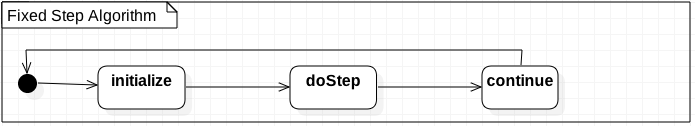
\includegraphics[width=3.5in,height=0.8in]{fig/MA1.png}
			\label{sd_fixedstep}}
		\hfil
		\subfigure[Rollback algorithm]{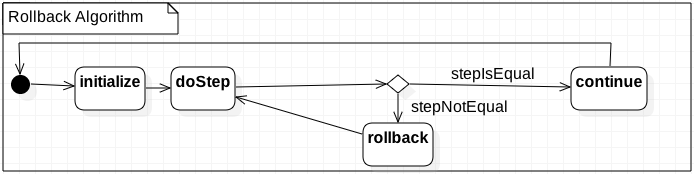
\includegraphics[width=3.5in,height=0.9in]{fig/MA2.png}
			\label{sd-rollback}}	
		\subfigure[Predictable step sizes algorithm]{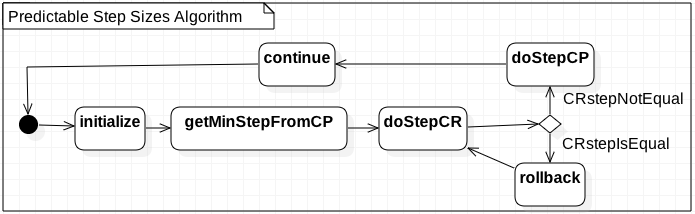
\includegraphics[width=3.5in,height=1.1in]{fig/MA3.png}
			\label{sd-pre}}		
	\caption{Activity diagrams for three versions of master algorithms.}
	\label{ad-fixedstep}
	}
\end{figure}
\subsubsection{Fixed Step Algorithm}
For fixed step algorithm, all FMUs have the same step size. When master algorithm calls \emph{doStep} with the step size \emph{h}, it will advance from a communication point \emph{t} to the next communication point \emph{t+h}. During the simulation step, an FMU with its own solver will simulate independently according to its input value and generate a running result as output value. MA will wait until all FMUs finish their simulation step and then get their output values to exchange data for preparing next simulation step. The activity diagram of fixed step algorithm is illustrated in Fig.\ref{sd_fixedstep}. There are mainly three activities in the control flow: \emph{initialize}, \emph{doStep} and \emph{continue}. In the fixed step algorithm \cite{BromanBGLMTW13}, the co-simulation process should be reliable, when all FMUs are reliable. When some error happens during a simulation step, the co-simulation will be affected due to the wrong simulation step. To overcome the shortcoming of the fixed step algorithm, it needs rollback mechanism.
\subsubsection{Rollback Algorithm}
There are some important features proposed in the FMI 2.0. It supports to save the FMU state if necessary and the saved state can be restored. For example, MA calls \emph{doStep} on $FMU_{1}$ and $FMU_{2}$ while $FMU_{1}$ can accept the request or $FMU_{2}$ can reject it. If we save the state of $FMU_{1}$ and $FMU_{2}$ at the communication point, we can restore the scene after $FMU_{2}$ rejects \emph{doStep}. The activity diagram of rollback algorithm is clearly shown in Fig.\ref{sd-rollback}. Compared with the fixed step algorithm, all FMUs are required to support \emph{rollback} mechanism, that is, all FMUs need to return to the previous state if the  step sizes of all FMUs simulation are not equal.
\subsubsection{Predictable Step Size Algorithm}
To improve the efficiency of MA, it is important to predict the step size. So, predictable step size algorithm is proposed. The function \emph{GetMaxStepSize} was introduced to optimize the performance of rollback algorithm. This function returns the maximum step size and state flag of a predictable FMU. Maximum step is the largest step that a predictable FMU can perform. State flag includes \emph{ok}, \emph{discard} and \emph{error}. \emph{OK} denotes the predictable FMU can accept the simulation step size. \emph{Discard} denotes the predictable FMU only implement partial step during simulation. \emph{Error} denotes the predictable FMU can't continue the simulation because of its unacceptable state or unreasonable input value. Also, when \emph{discard} and \emph{error} happen, the FMU needs to rollback to the previous saved state. Whether an FMU is a predictable FMU or not should be indicated in FMU's \emph{xml} file. Moreover, if an FMU supports rollback and predictable step size at the same time, the predictable step size algorithm only uses predictable ability to get the maximum step of a predictable FMU. On the other hand, a predictable FMU can accept any step size less than or equal to the maximum step returned by \emph{GetMaxStepSize}.

First, the master algorithm chooses the maximum step size of all predictable FMUs and find the smallest communication step size \emph{h} that all predictable step size can be accepted. Then, we save the states of all FMUs. MA calls \emph{doStep(h)} on FMUs supporting rollback. The function \emph{doStep()} will return the real performed step size. If all performed step sizes are equal to \emph{h}, MA will call \emph{doStep(h)} on FMUs. Otherwise, MA will find the smallest performed step $h_{min}$, then all FMUs will restore the state saved before the co-simulation. Finally, MA will invoke $doStep$ $(h_{min})$ on all FMUs. The control flow of predictable step size algorithm is shown in Fig.\ref{sd-pre}. For example, \emph{getMinStepFromCP} is an activity that MA will call \emph{GetMaxStepSize} on all predictable FMUs to find their maximum simulation step size and then return the smallest one of them. 

\subsection{Modelling and Analysis of MA} 
UPPAAL \cite{BehrmannDLHPYH06} is a toolset for verification of real-time systems represented by (a network of) timed automata which is extended with integer variables, structured data types, and channel synchronization. We model the master algorithms using timed automata in UPPAAL. The Fig.\ref{ta-master} shows the timed automata models of three master algorithms,  respectively. Fixed step algorithm has \emph{Init}, \emph{doStep} states and synchronize with \emph{FMU} by channel \emph{continue}. Rollback algorithm has \emph{Init}, \emph{DoStep}, and \emph{Continue} states. If all FMUs don't have the same step size, rollback algorithm will communicate with FMUs by \emph{rollback} signal, otherwise, it will send \emph{continue} signal and move to \emph{Continue} state. Predictable step size algorithm has \emph{Init}, $find \_ CP \_ MIN$, \emph{DoStep}, \emph{writeCP} states. It obtains the minimal step size (i.e., \emph{step2}) of FMUs supporting \emph{GetMaxStepSize} function and the maximal step size (i.e., \emph{step1}) of FMUs supporting rollback. If \emph{step1} is greater than \emph{step2}, FMUs receive \emph{rollback} signal and return to \emph{DoStep} state. Otherwise, FMUs receive \emph{continue} signal and do the next step.  



\begin{figure}[htbp]
\centering{
		\subfigure[Timed automata for fixed step algorithm]{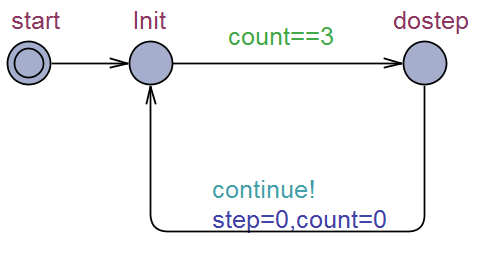
\includegraphics[width=1.0in,height=0.8in]{fig/fixedstep_master.png}
			\label{ta_fixedstep}}
		\hfil
		\subfigure[Timed automata for rollback algorithm]{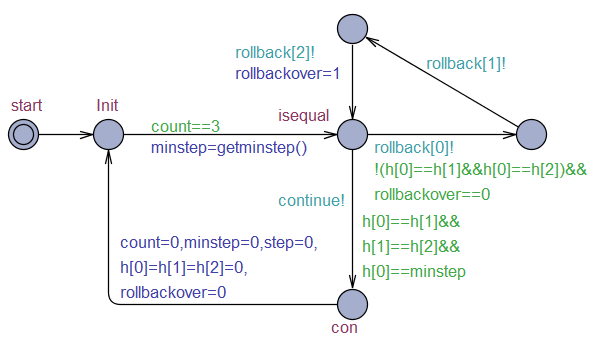
\includegraphics[width=2.0in,height=1.2in]{fig/rollback_master.png}
			\label{ta-rollback}}	
		\subfigure[Timed automata for predictable step size algorithm]{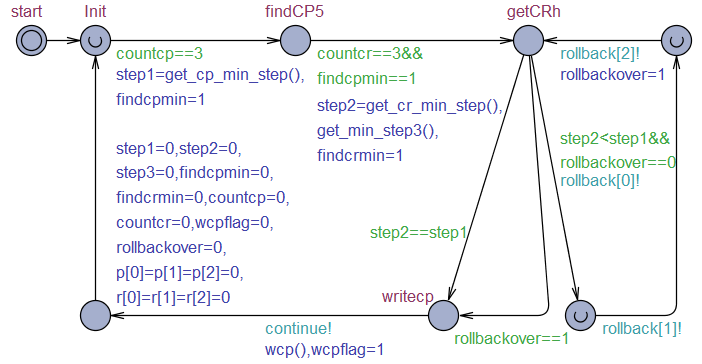
\includegraphics[width=3.5in,height=1.6in]{fig/pma_master.png}
			\label{ta-pre}}		
	\caption{Timed automata for three versions of master algorithms.}
	\label{ta-master}
	}
\end{figure}


 
We verify the properties of master algorithms including reachability, liveness and deadlock. Experimental results are shown in Table \ref{ta_r}, where:

\begin{itemize}
\item
$E \langle\rangle ~master.dostep$, $E\langle\rangle~master.Continue$ and $E\langle\rangle~master.writeCP$ are reachability properties checking whether the model can reach these states;
\item
$master.Init \rightarrow master.dostep$, $master.Init \rightarrow master.Continue$ and $master.Init \rightarrow master.Continue$ are liveness property. If the master algorithm arrives at the former state, it eventually reaches the latter state;
\item
$A[]~not~deadlock$ is safety property, which means whether the model will be deadlock.
\end{itemize}

In Table \ref{ta_r}, we can find that the properties such as deadlock, liveness and reachability are satisfied,  which proves that the correctness of co-simulation behavior. For example, $A[]~not~deadlock$ is satisfied, which means the MA is deadlock free. $master.Init \rightarrow master.doStep$ is satisfied, which means if the model reach the former state $Init$, it will eventually reach the state $doStep$. $E\langle\rangle~master.doStep$ is satisfied, which means there exists a reachable state $doStep$. 

\begin{table}
\caption{Experimental results for verifying MA}
\centering
\begin{tabular}{c c c}
        \hline
        MA & Property & Result\\
        \hline
        \multirow{2}{2.0cm}{Fixed Step}
                & $A[]~not~deadlock$ & True\\
                & $master.Init \rightarrow master.dostep$ & True\\
                & $E\langle\rangle~master.dostep$ & True\\

        \hline
        \multirow{2}{2.0cm}{Rollback}
                & $A[]~not~deadlock$ & True\\
                & $master.Init \rightarrow master.Continue$ & True\\
                & $E\langle\rangle~master.Continue$ & True\\

        \hline
        \multirow{2}{2.0cm}{Predictable}
                & $A[]~not~deadlock$ & True\\
                & $master.Init \rightarrow  master.writeCP$ & True\\
                & $E\langle\rangle~master.writeCP$ & True\\
        \hline
\end{tabular}
\label{ta_r}
\end{table}



\section{Case study}
\label{sec:sysml}
To illustrate our approach, we take an example water tank as the case study inspired by \cite{AmalioPCW16}. According to the I/O dependency information between FMUs, the architectural model for water tank is constructed using SysML BDD, which helps to model the components and their connections.

%\subsection{Case Study: Water Tank}
The water tank system is shown in Fig.~\ref{tankfig}. A source of water flows into the water tank whose water flows into the drain. The source is controlled by a valve. When the valve is open, the water flows into the water tank. The valve, managed by a software controller, is opened or closed stochastically depending on the water level. In this paper, we illustrate three various version of water tank systems to show the scability of our approach. The difference between various water tank cases lies in various connection way between the controller, valve and tank. 
\begin{figure}[htbp]
	\centering	{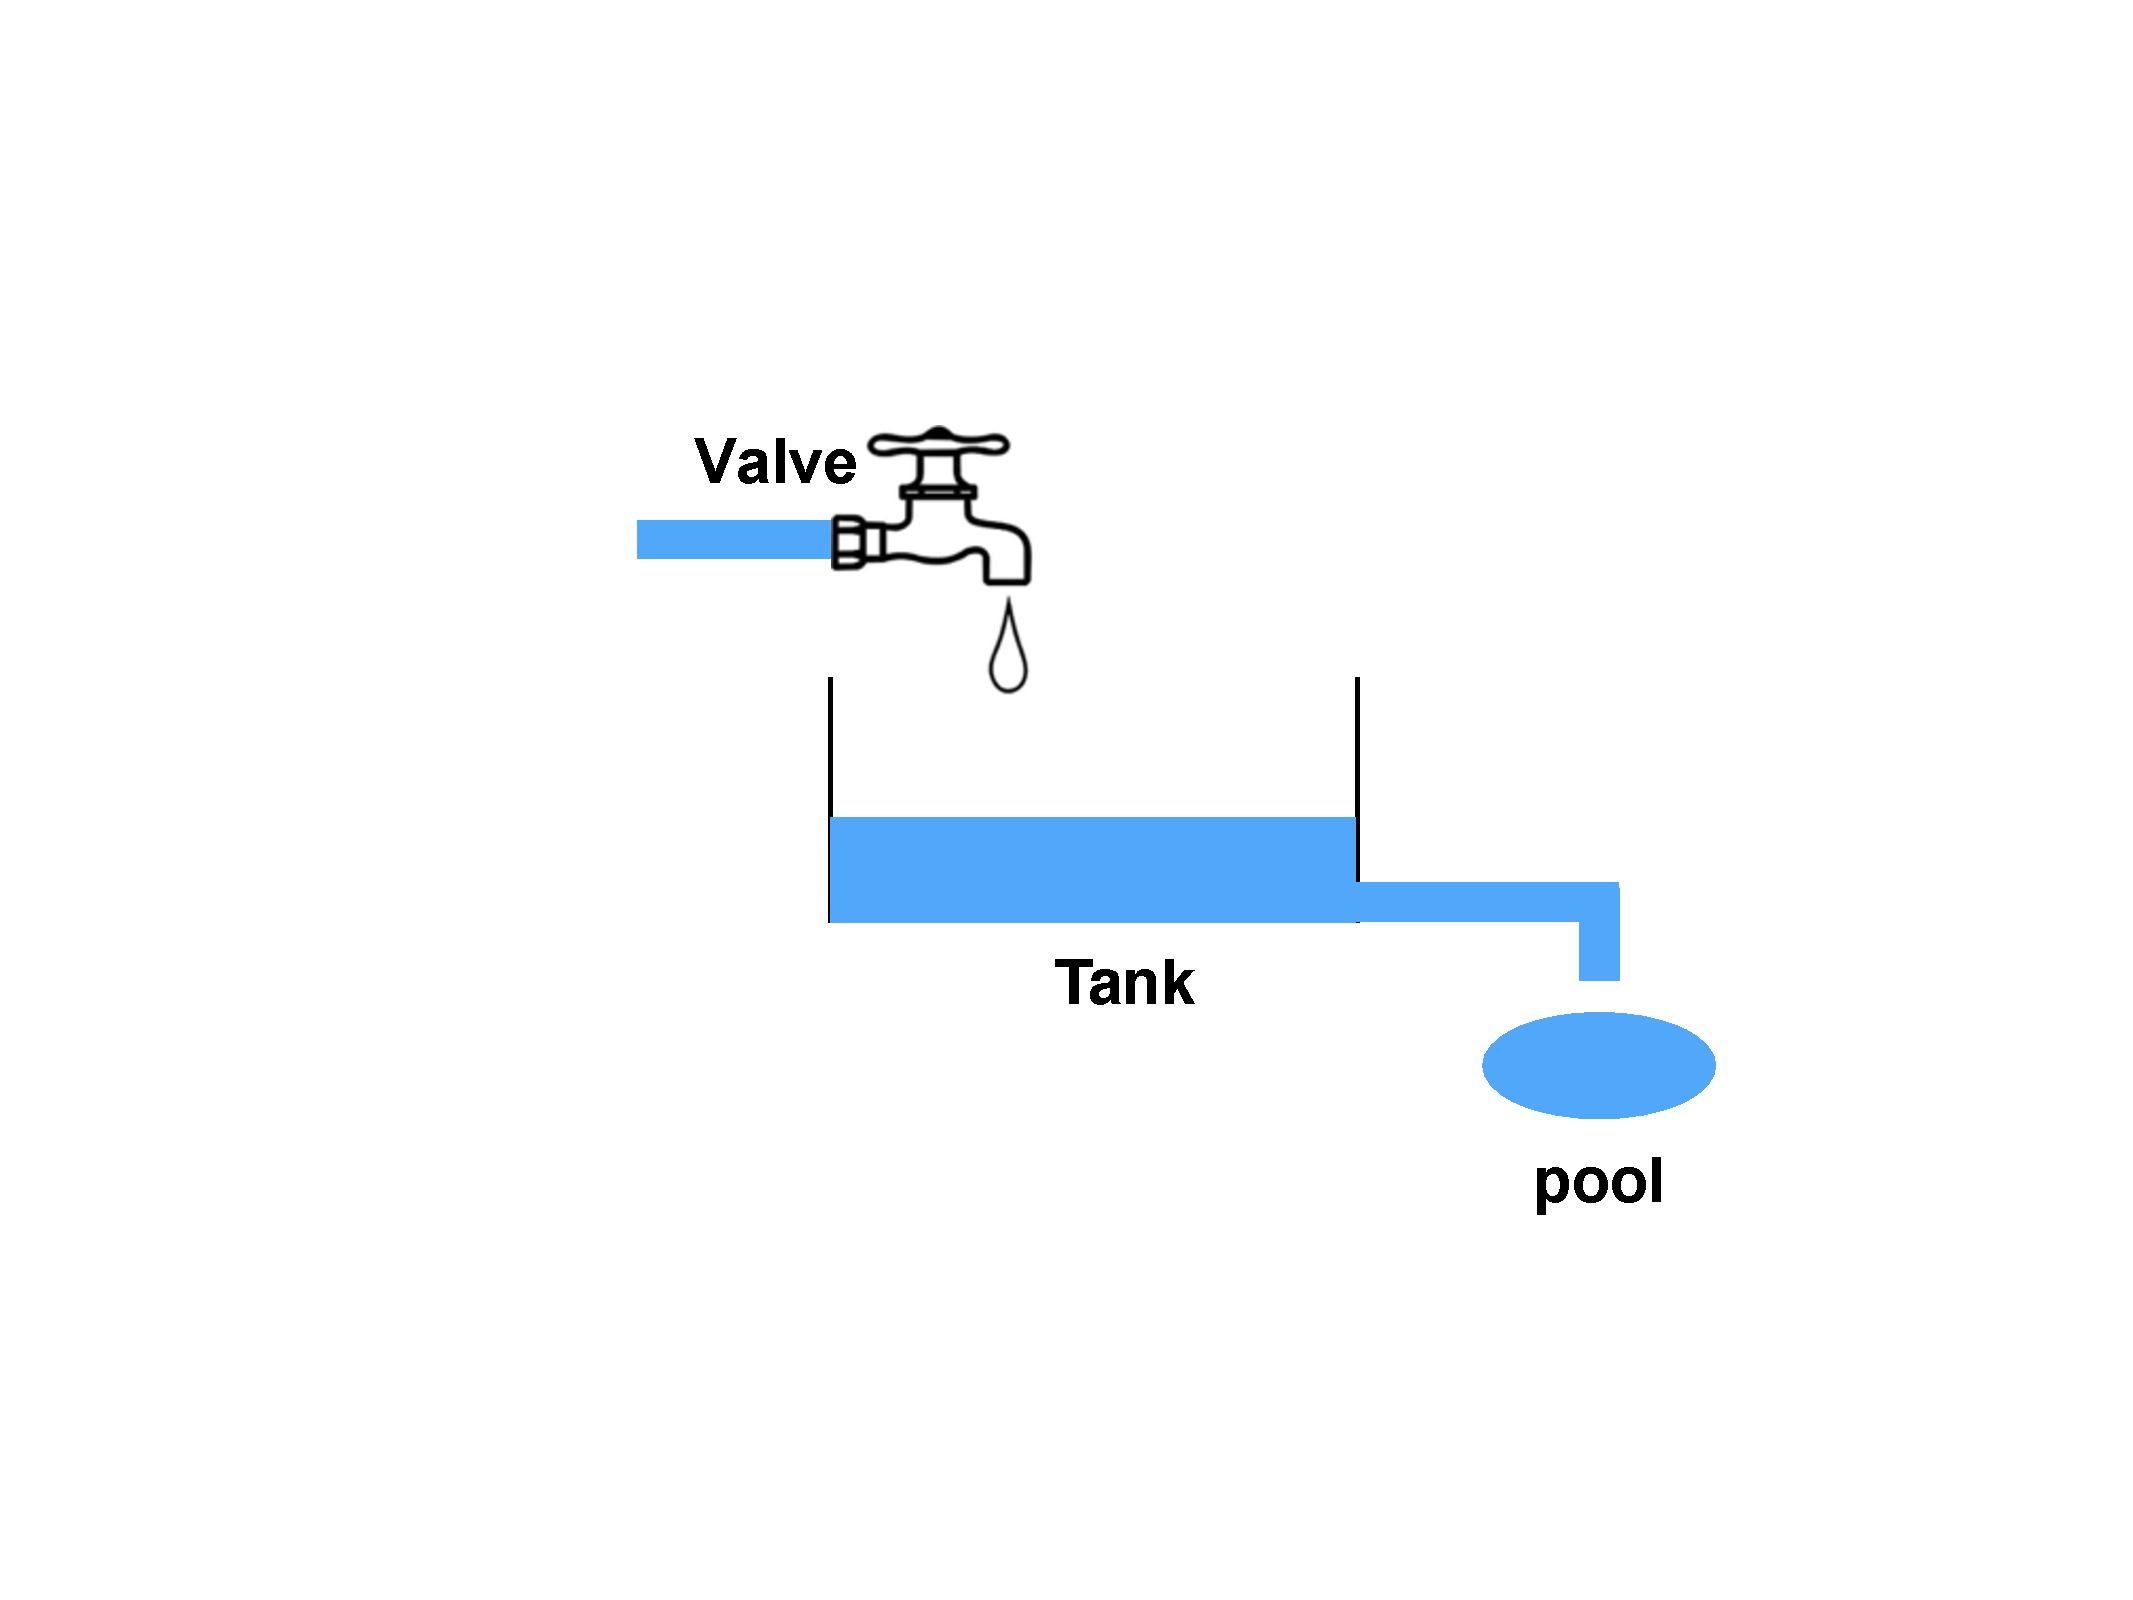
\includegraphics[width=1.7in,height=1.2in]{fig/tank-fig.pdf}}
	\caption{Water tank system.}
	\label{tankfig}
\end{figure} 
\subsection{Architecture Modeling with SysML}
SysML is a general purpose Domain-Specific Language (DSL) \cite{SemerathBHSV17} for Model-Based Systems Engineering (MBSE) \cite{Dori16}, which is originated as an initiative of the International Council on Systems Engineering (INCOSE) \cite{Pepper2015International} in January 2001. The SysML BDD describes the structure of the system with blocks. The IBD describes the internal structure and connections of blocks. The ports of blocks are connected by the connector. The I/O dependence of blocks describes the communication between blocks. SysML BDD is usually used to model the architecture of system.

Fig.~\ref{myad} shows the SysML BDD for the water tank system, which consists of three blocks: $Valve$, $Tank$ and $Controller$. $Valve$ and $Tank$ are physical components. $Controller$ is the cyber component. Each component has its own input and output. For instance, the input interface of $Valve$ is named as $vin$, which is used to input the $OpenClosed$ signal. 
\begin{figure}[htbp]
	\centering	{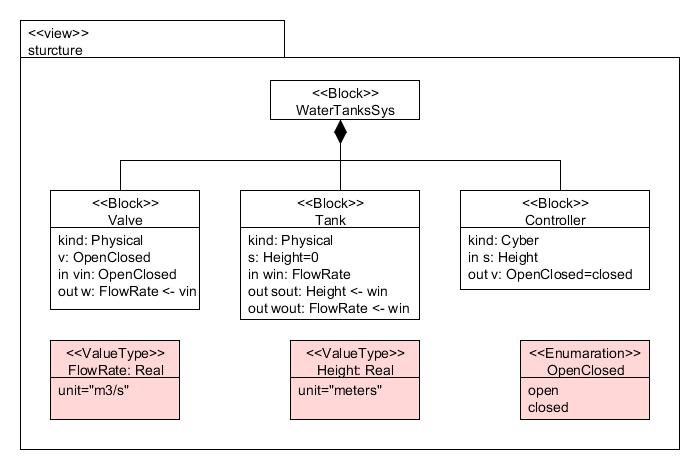
\includegraphics[width=3.2in,height=2.3in]{fig/AD.jpg}}
	\caption{SysML BDD for water tank.}
	\label{myad}
\end{figure}

Fig.~\ref{cd} shows the connection diagram for the system. There are three cases for connections. The first case is that the system has one valve, one controller and one tank. The controller sends stochastic signals to control the valve on/off leading to various rates of water flow. The second case is that the signal from the controller is affected by the water level of the tank. The last case is modified based on the first case and added another $waterTank2$ which is affected by the flow rate of the $waterTank1$.

\begin{figure}[htbp]
\centering{
		\subfigure[Connection case 1]{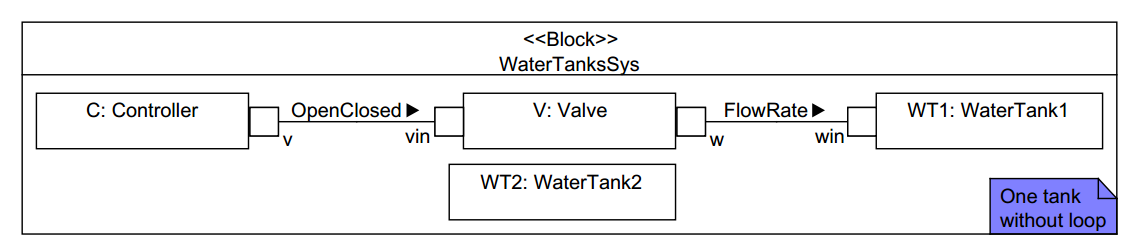
\includegraphics[width=3.2in,height=0.8in]{fig/CD1.png}
			\label{cd1}}
		\hfil
		\subfigure[Connection case 2]{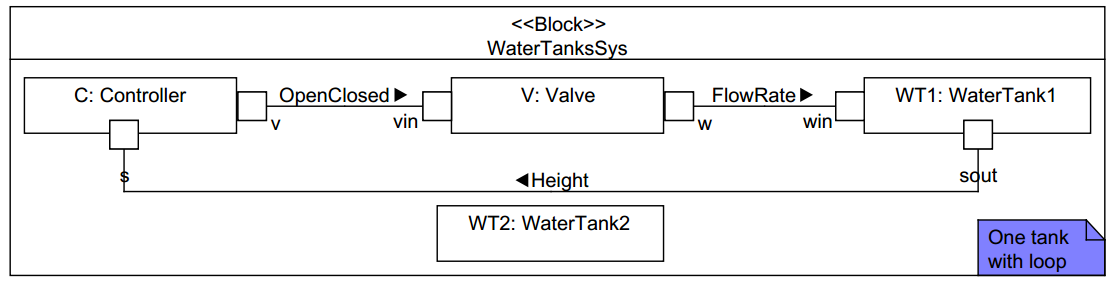
\includegraphics[width=3.2in,height=0.8in]{fig/CD2.png}
			\label{cd2}}
		\hfil
		\subfigure[Connection case 3]{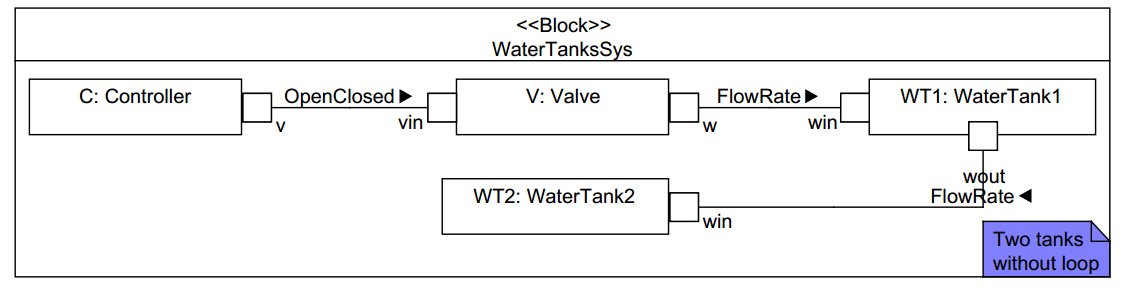
\includegraphics[width=3.2in,height=0.8in]{fig/CD3.png}
			\label{cd3}}
	\caption{SysML IBD for water tank.}
	\label{cd}
	}
\end{figure}
The SysML BDD shows the blocks of system and SysML IBD shows the connection between blocks. In next section, we abstract each block as an FMU, and model SysML IBD as the connector configuration.

\subsection{FMUs Connection of Water Tank}
Fig.~\ref{fmu-con} is the FMUs and FMUs connection of water tank system. There are three connection cases between the FMUs according to the SysML IBD shown in Fig.~\ref{cd}. The first case contains three FMU components $Controller$, $Valve$ and $WaterTank1$ and two channels $v \_ vin$, $w \_ win$ as shown in Fig.\ref{fmu-con1}. The $Controller$ and $Valve$ are connected with channel $v \_ vin$. The $Valve$ and $WaterTank1$ are connected with channel $w \_ win$. The second case is shown in Fig.\ref{fmu-con2}, there could be a channel $sout \_ s$ between $WaterTank1$ and $Controller$, which means the water level of $WaterTank1$ affects the control strategy of the \textbf{controller}. Fig.~\ref{fmu-con3} shows the third case, there could be another $WaterTank2$, the $WaterTank1$ and $WaterTank2$ are connected by the channel $w \_ out$. 
\begin{figure}[htbp]
\centering{
		\subfigure[Case 1]{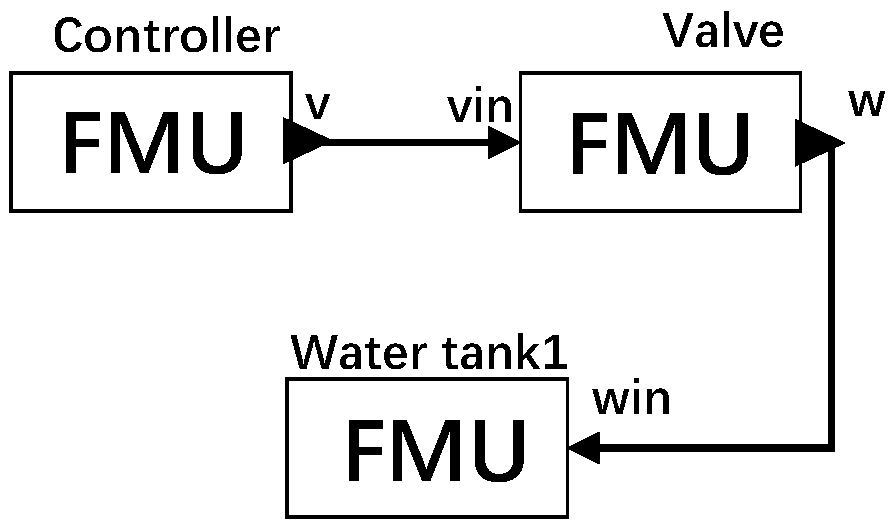
\includegraphics[width=1.0in,height=0.6in]{fig/fmuc1.png}
			\label{fmu-con1}}
		\hfil
		\subfigure[Case 2]{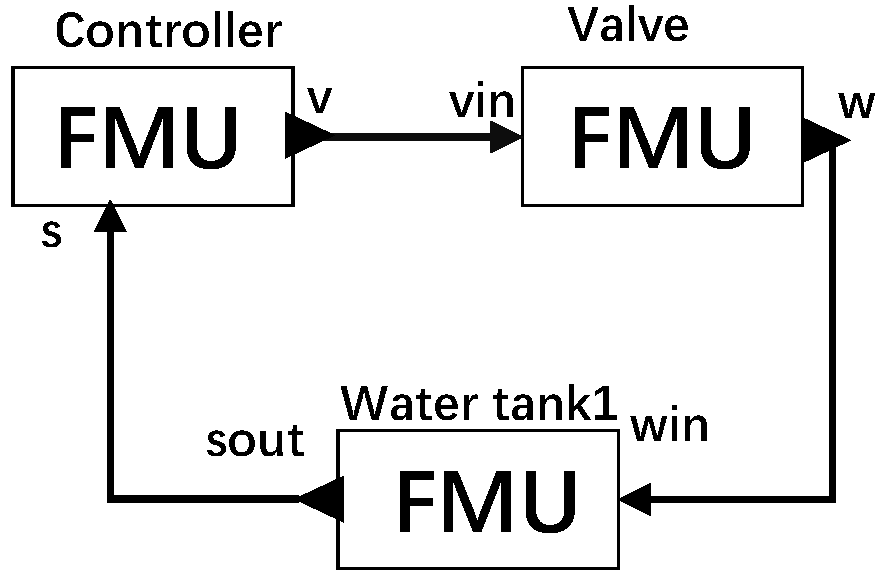
\includegraphics[width=1.0in,height=0.6in]{fig/fmuc2.png}
			\label{fmu-con2}}
		\hfil
		\subfigure[Case 3]{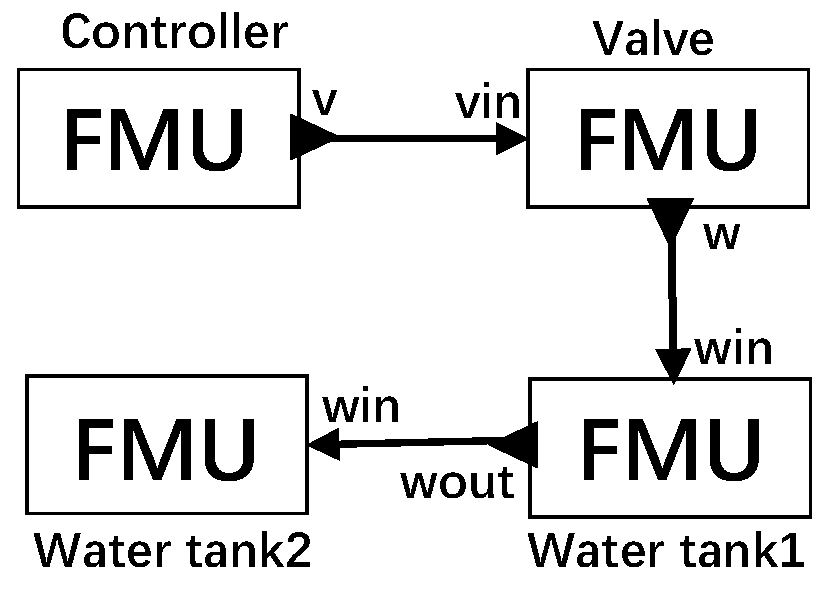
\includegraphics[width=1.0in,height=0.6in]{fig/fmuc3.png}
			\label{fmu-con3}}
	\caption{FMUs connections of three water tank cases.}
	\label{fmu-con}
	}
\end{figure}

Until now, we design the architecture and the connections of the case study. Before the system is co-simulated in the engine, how can we assure the correctness of the architecture models? To solve this problem, we use model checking to verify it. This is one of our main contributions. More details of verification process can be found in the next section.
\subsection{Verification and Analysis with UPPAAL}
\label{sec:mauppaal}
This section performs a formal analysis of the architectures of water tank. First of all, we encode FMUs of the water tank and model the MA with TA which composes a network of TA. Next, the models are verified with the model checker UPPAAL. The execution of FMU and co-simulation is time-related. We abstract the execution of FMUs for the water tank and encode it with the locations and transitions of TA according to the encoding rules proposed in Section \ref{sec:encoding}. Besides, we also model the MA as a TA to coordinate the execution between several FMUs. The TA templates for FMUs and MA are shown in Fig.\ref{tk-arch1}. Here, we adopt the rollback MA to coordinate the FMUs. The other two MAs can be analysed with the similar way. We do not present the details of them due to the space limits of this paper.

\begin{figure}[htbp]
\centering{
		\subfigure[TA for FMU\_controller]{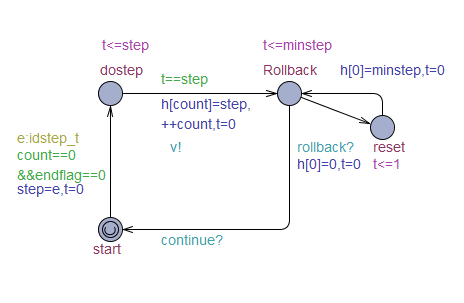
\includegraphics[width=1.6in,height=1.0in]{fig/2signal_controller.png}
			\label{tk_controller}}
		\hfil
		\subfigure[TA for FMU\_valve]{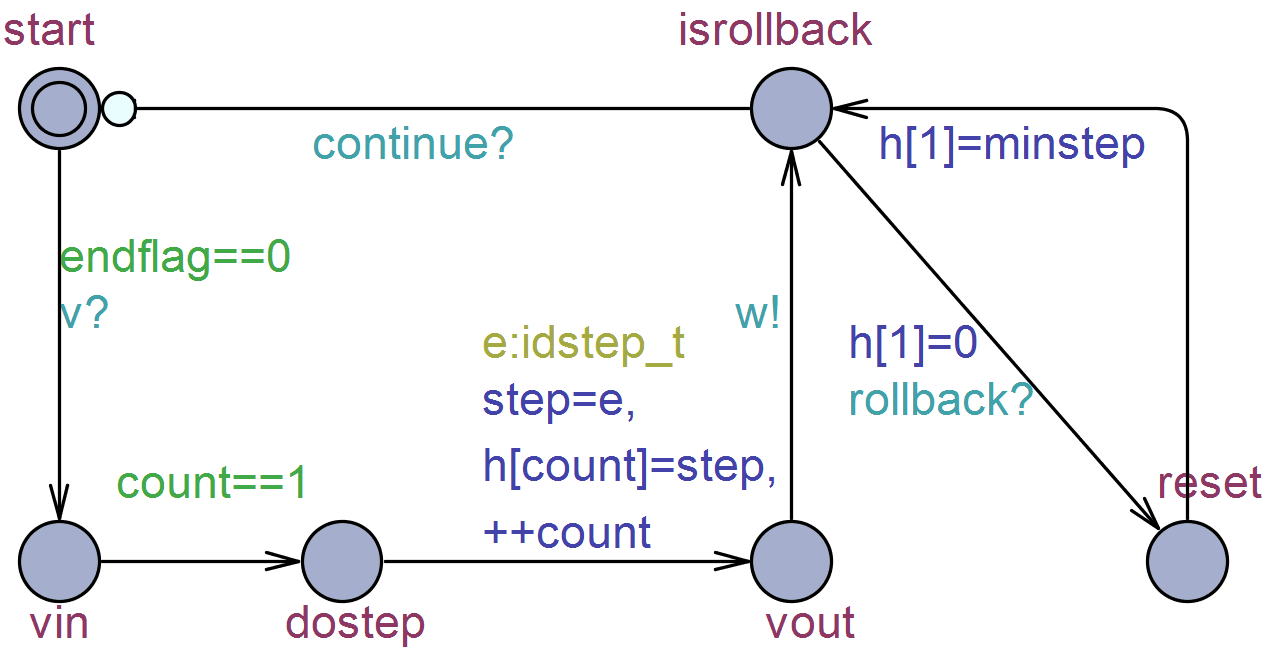
\includegraphics[width=1.6in,height=1.0in]{fig/2signal_v.png}
			\label{tk_v}}
			
	    \subfigure[TA for FMU\_WaterTank1]{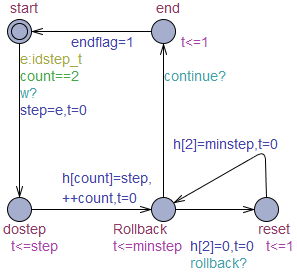
\includegraphics[width=1.5in,height=1.2in]{fig/2signal_wt1.png}
			\label{tk_wt1}}
		\hfil
		 \subfigure[TA for rollback MA]{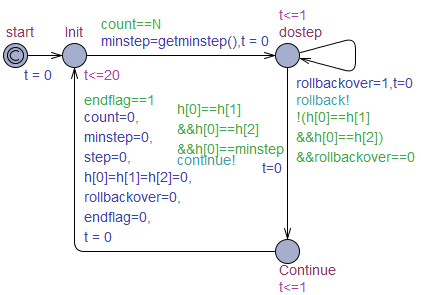
\includegraphics[width=1.7in,height=1.2in]{fig/2signal_master.png}
			\label{tk_ma}}		
	\caption{TA Network for connection case 1: $controller$ $\vert\vert$ $valve$ $\vert\vert$ $WaterTank1$ $\vert\vert$ $MA$.}
	\label{tk-arch1}
	}
\end{figure}

\begin{figure}[htbp]
\centering{
		\subfigure[Execution trace]{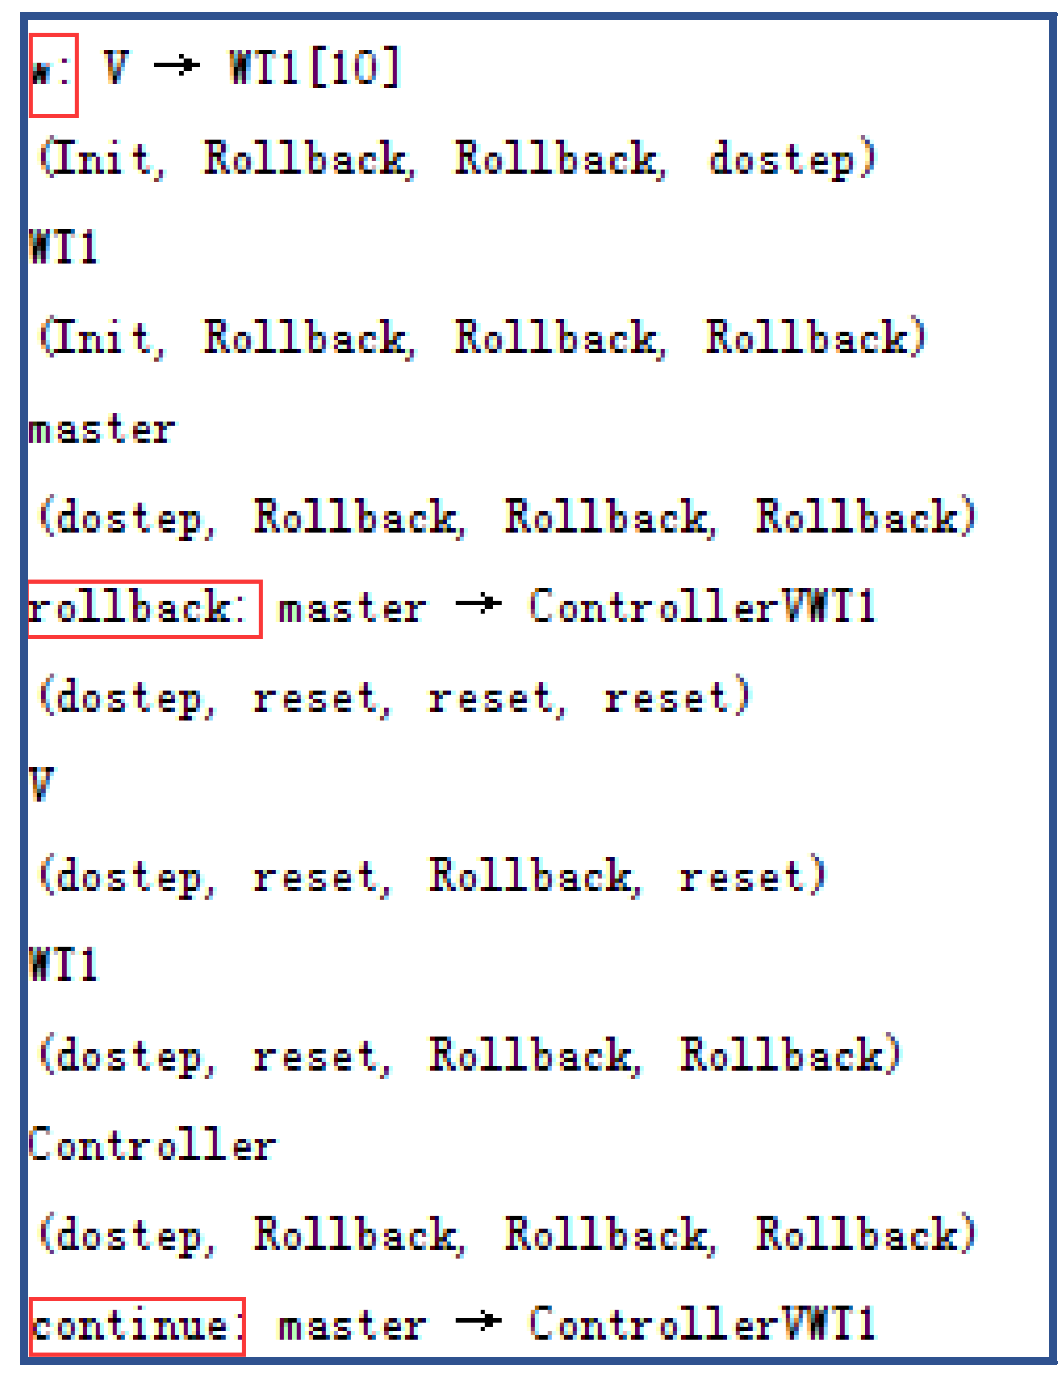
\includegraphics[width=1.6in,height=1.8in]{fig/trs.png}
			\label{trs}}
		\hfil
		\subfigure[Execution sequence diagram]{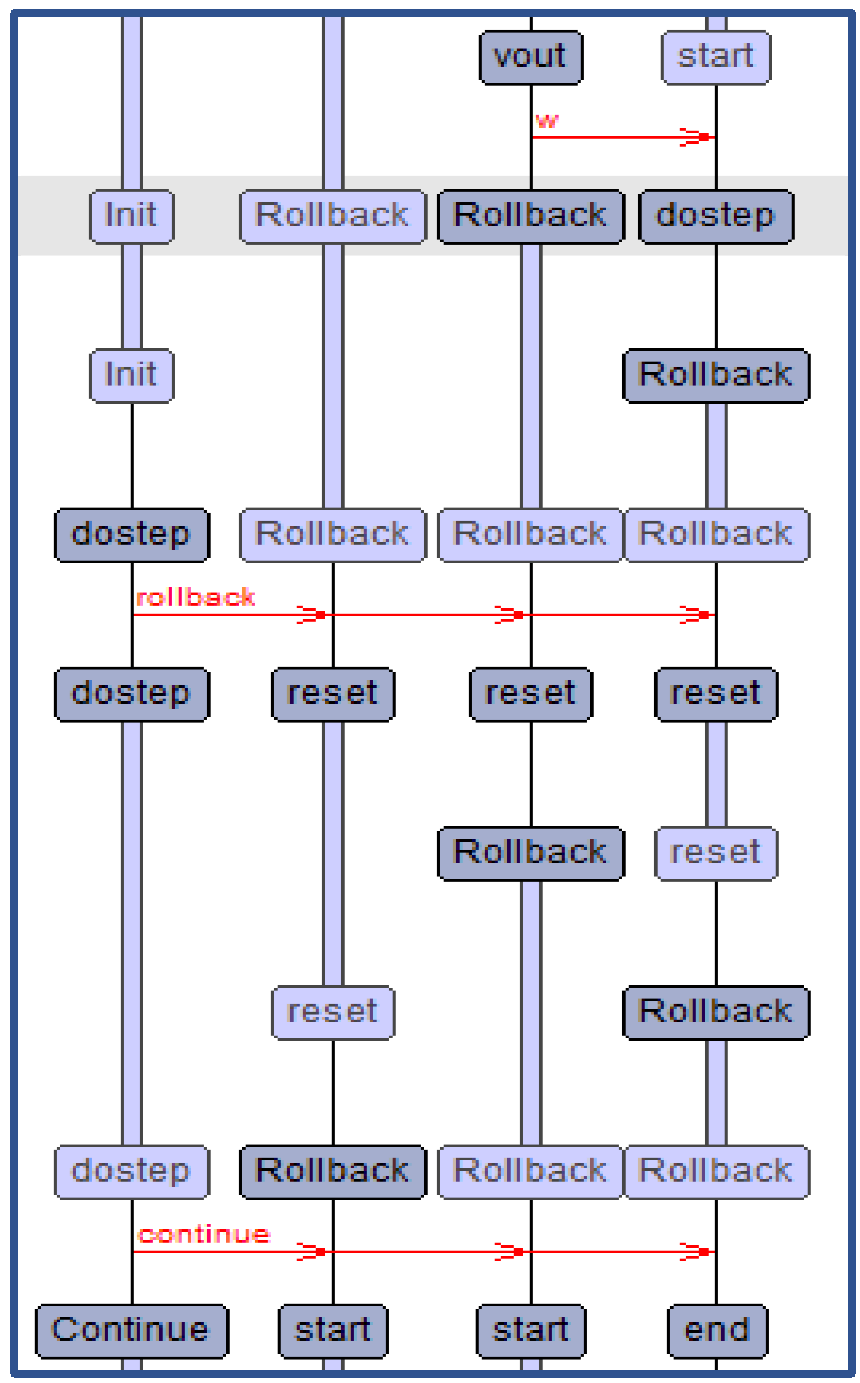
\includegraphics[width=1.6in,height=1.8in]{fig/seq.png}
			\label{seq}}
	\caption{The execution fragment of the coordination in UPPAAL.}
	\label{trs-seq}
	}
\end{figure}

Fig.~\ref{tk_controller}, \ref{tk_v}, \ref{tk_wt1} are the templates for $controller$, $valve$ and $WaterTank1$ respectively, which model FMUs of the water tank. These FMUs have four key states: $start$, $dostep$, $Rollback$ and $reset$. Fig.~\ref{tk_controller} shows the template for $controller$ which executes with the random step size. It synchronizes with $valve$ by signal $v$ and transfers to $Rollback$ state, and then waits for a signal from the MA. Until the $controller$ receives the $continue$ signal, it does data exchange with other FMUs, and returns to $start$ state. Otherwise, it receives $rollback$ signal, when it obtains the minimize step size of all FMUs, it transfers to $Rollback$ state. The states and transitions of $valve$ and $WaterTank1$ template are similar with the template of $controller$. Fig.~\ref{tk_ma} shows the template for the MA. Firstly, the MA initializes the parameters, and then it gets minimize step size of FMUs until all FMUs visit $dostep$. Next, the MA decides which signal should be sent according to the guard. If the step sizes of all FMUs are equal, the MA will send $continue$ signal, otherwise, send $rollback$ signal.

Fig.~\ref{trs-seq} is the execution fragment of the coordination in UPPAAL, we can find that $valve$ sends a $w$ signal to perform data exchange with $WaterTank1$. After that, $WaterTank1$ moves to $dostep$ state. The MA broadcasts a $rollback$ signal to all templates, which leads to all of them arrive at $reset$ state. Finally, the MA sends a $continue$ signal to all FMUs. All templates return to $start$ state, and then do the next step. The execution fragments show that our models are correct.

In order to compare the behavior of three connection cases of water tank system, we also model the other two connection cases in UPPAAL. For connection case 2, we add channel $s$ in the templates for $controller$ and $WaterTank1$ as shown in Fig.\ref{tk-arch2}. For connection case 3, we create template for $WaterTank2$ and channel $w2$ as shown in Fig.\ref{arc3}. The other models are the same as models of connection case1. Limited to the length of this paper, we only show the templates for $controller$ and $WaterTank1$ of connection case 2 and template for $WaterTank2$ of connection case 3. In the next subsection, we verify some properties of various connection cases to detect whether there is an algebraic loop in the architecture.
\begin{figure}[htbp]
\centering{
		\subfigure[TA for FMU\_controller]{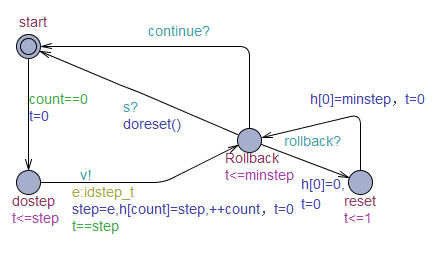
\includegraphics[width=1.8in,height=1.2in]{fig/2signal_cycle_controller.png}
			\label{tk2_controller}}
		\hfil
		\subfigure[TA for FMU\_WaterTank1]{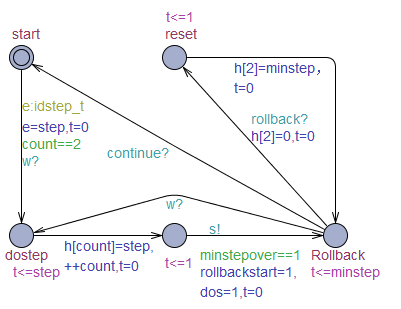
\includegraphics[width=1.5in,height=1.2in]{fig/2signal_cycle_wt1.png}
			\label{tk2_v}}		
	\caption{TA for connection case 2.}
	\label{tk-arch2}
	}
\end{figure}
\begin{figure}[htbp]
	\centering	{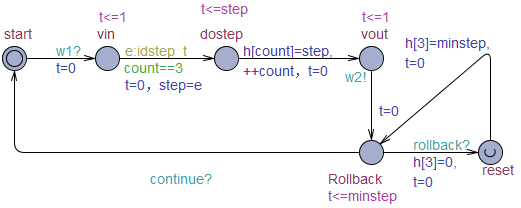
\includegraphics[width=3.5in,height=1.2in]{fig/4signal_wt2.png}}
	\caption{TA for FMU\_WaterTank2 of connection case 3.}\label{arc3}
\end{figure}

UPPAAL supports a simplified version of TCTL \cite{BouchenebGR09} to specify the property. We verify the following properties of each connection case:
\begin{itemize}
\item
$E\langle\rangle~WT1.Rollback$ and $E\langle\rangle~master.Continue$ specify reachability properties. It means the FMU of $WaterTank1$ will $Rollback$ and the MA will reach $Continue$ state.
\item
$master.start \rightarrow master.Continue$ specifies liveness property. It means once the MA start, it will continue eventually.
\item 
$A[]~not~deadlock$ specifies safety property. It means the execution of the system will not be deadlock.
\end{itemize}

The verification results are listed in Table \ref{rs}. We can find that all properties of connection case 1 and case 3 are satisfied. It shows that our MA works well and the composition of FMUs is determinate. However, the liveness and reachability properties of connection case 2 are not satisfied. It means there is an algebraic loop which may be introduced with the I/O dependency in the architecture. The experimental results show that our approach is feasible and useful for model checking the coordination of CPS. Here, we only focus on the detection of algebraic loop and the correctness of coordination. In the future work, we will consider how to eliminate the algebraic loop.  
\begin{table}
\caption{Experimental results for various connection case}
\centering
\begin{tabular}{c c c} 
        \hline  
        Connection case & Verified Property & Result\\
        \hline
        \multirow{2}{2.0cm}{Case 1}  
                & $E\langle\rangle~WT1.Rollback$ & True\\ 
                & $E\langle\rangle~master.Continue$ & True\\ 
                & $master.start\rightarrow master.Continue$ & True\\ 
                & $A[]~not~deadlock$ & True\\   
        \hline 
        \multirow{2}{2.0cm}{Case 2}  
                & $E\langle\rangle~WT1.Rollback$ & True\\ 
                & $E\langle\rangle~master.Continue$ & False\\ 
                & $master.start\rightarrow master.Continue$ & False\\ 
                & $A[]~not~deadlock$ & True\\   
        \hline 
        \multirow{2}{2.0cm}{Case 3}  
                & $E\langle\rangle~WT1.Rollback$ & True\\ 
                & $E\langle\rangle~master.Continue$ & True\\ 
                & $master.start \rightarrow master.Continue$ & True\\ 
                & $A[]~not~deadlock$ & True\\   
        \hline 
\end{tabular} 
\label{rs}
\end{table}





\section{Related Works}
Statistical Model Checking technique was first proposed by R.Grosu \cite{grosu2005monte}. Some variations \cite{legay2010statistical} \cite{Younes2004Planning} \cite{younes2006statistical}\cite{jha2009bayesian} \cite{zuliani2013bayesian} \cite{herault2004} based on the basic SMC have been proposed in the past few years. Some related work are summarized as follows:

\textbf{Basic SMC.}
SMC refers to a series of simulation-based techniques that can be used to answer two questions: (1)Qualitative: Is the probability of model \emph{s} satisfying property $\phi$ greater than or equal to a certain threshold? and (2)Quantitative: What is the probability of model \emph{s} satisfying property $\phi$? For qualitative SMC, Kim.G.larsn et al. \cite{kim2012statistical} have given an empirical evaluation. BHT and SPRT are more effective than SSP. BHT generates more traces when checking the property whose estimation probability is close to its real probability, so SPRT is faster than BHT for this situation. For other situation, BHT is obviously more efficient than SPRT. For quantitative SMC, Zuliani et al. \cite{zuliani2013bayesian} have compared the number of traces analyzed by APMC and BIE, and they have concluded that BIE excels remarkably in performance. Our approach focuses on the performance of BIE algorithm.

\textbf{SMC with abstraction and learning.}
BIE algorithm needs more traces when checking the property whose probability is close to 0.5, while the number of traces is drastically reduced when the probability approaches to 0 or 1 \cite{zuliani2013bayesian}. In our recent work \cite{jiangkaiqiang2016}, we have partitioned the original probability space $\Omega$ into many sub-spaces $\Omega_1$,... ,$\Omega_m$, and evaluated the probability of each sub-space in parallel. Therefore, the trace number for evaluating the original probability will be decreased and depends on the maximum number of traces for evaluating sub-spaces theoretically. We find that the number of traces is effectively reduced while ensuring the accuracy of the probability within an acceptable error bound.

\textbf{Distributed SMC.}
As observed in \cite{younes2005ymer}, SMC algorithms can be distributed with master/slave architecture where multiple slave processes are used to generate traces. When working with an estimation algorithm, the number of traces for verifying the property is known in advance and can be equally distributed between the slaves. When working with the sequential algorithms, the situation gets more complicated, so we need to avoid introducing bias when collecting the traces generated by the slave processes. To solve this problem, H. L. S. Younes proposed a method in \cite{Younes2004Planning} where the bias is avoided by committing ,$\alpha$ $priori$, to the order in which observations will be taken into account. Peter Bulychev et al. generalized the above method with batches and buffer \cite{Bulychev2012Checking}. Batches aggregate the outcomes for reducing communication and the buffer is used to improve concurrency since the nodes are more loosely synchronized. They also implemented the distributed Hypothesis testing algorithm without introducing bias. The algorithm effectively reduce the time consumption for generating a single trace. Our work is different from the existing work, we use abstraction and learning technique (AL-SMC) to reduce the number of simulation traces, and adopt distributed technology with AL-SMC to reduce both the number of traces and time consumption for generating a single traces.   
\section{Conclusion and Future Work}
\label{sec:conclusion&ack}
This paper has presented our novel approach to check the FMI co-simulation , which facilitates the formal analysis of CPSs. This involves model checking the reachability, livelock and deadlock of three various master algorithms. Besides, the correctness and  relevant system properties of the architecture are also analysed. To achieve the goal, we encode the FMU and master algorithms with timed automata. Then the properties of the co-simulation are verified with UPPAAL. We evaluate this approach using the example water tank. The results show that our approach is feasible and useful.

An interesting direction of future work is that we attempt to analyse and compare the performance of various master algorithms in the future. Besides, more complex case studies will be conducted to check the scalability of proposed approach. The tool support for our approach should be improved further.
\section*{Acknowledgement}
This work was supported by NSFC (Grant No.61472140, 61202104) and NSF of Shanghai (Grant No. 14ZR1412500).





% An example of a floating figure using the graphicx package.
% Note that \label must occur AFTER (or within) \caption.
% For figures, \caption should occur after the \includegraphics.
% Note that IEEEtran v1.7 and later has special internal code that
% is designed to preserve the operation of \label within \caption
% even when the captionsoff option is in effect. However, because
% of issues like this, it may be the safest practice to put all your
% \label just after \caption rather than within \caption{}.
%
% Reminder: the "draftcls" or "draftclsnofoot", not "draft", class
% option should be used if it is desired that the figures are to be
% displayed while in draft mode.
%
%\begin{figure}[!t]
%\centering
%\includegraphics[width=2.5in]{myfigure}
% where an .eps filename suffix will be assumed under latex, 
% and a .pdf suffix will be assumed for pdflatex; or what has been declared
% via \DeclareGraphicsExtensions.
%\caption{Simulation results for the network.}
%\label{fig_sim}
%\end{figure}

% Note that the IEEE typically puts floats only at the top, even when this
% results in a large percentage of a column being occupied by floats.


% An example of a double column floating figure using two subfigures.
% (The subfig.sty package must be loaded for this to work.)
% The subfigure \label commands are set within each subfloat command,
% and the \label for the overall figure must come after \caption.
% \hfil is used as a separator to get equal spacing.
% Watch out that the combined width of all the subfigures on a 
% line do not exceed the text width or a line break will occur.
%
%\begin{figure*}[!t]
%\centering
%\subfloat[Case I]{\includegraphics[width=2.5in]{box}%
%\label{fig_first_case}}
%\hfil
%\subfloat[Case II]{\includegraphics[width=2.5in]{box}%
%\label{fig_second_case}}
%\caption{Simulation results for the network.}
%\label{fig_sim}
%\end{figure*}
%
% Note that often IEEE papers with subfigures do not employ subfigure
% captions (using the optional argument to \subfloat[]), but instead will
% reference/describe all of them (a), (b), etc., within the main caption.
% Be aware that for subfig.sty to generate the (a), (b), etc., subfigure
% labels, the optional argument to \subfloat must be present. If a
% subcaption is not desired, just leave its contents blank,
% e.g., \subfloat[].


% An example of a floating table. Note that, for IEEE style tables, the
% \caption command should come BEFORE the table and, given that table
% captions serve much like titles, are usually capitalized except for words
% such as a, an, and, as, at, but, by, for, in, nor, of, on, or, the, to
% and up, which are usually not capitalized unless they are the first or
% last word of the caption. Table text will default to \footnotesize as
% the IEEE normally uses this smaller font for tables.
% The \label must come after \caption as always.
%
%\begin{table}[!t]
%% increase table row spacing, adjust to taste
%\renewcommand{\arraystretch}{1.3}
% if using array.sty, it might be a good idea to tweak the value of
% \extrarowheight as needed to properly center the text within the cells
%\caption{An Example of a Table}
%\label{table_example}
%\centering
%% Some packages, such as MDW tools, offer better commands for making tables
%% than the plain LaTeX2e tabular which is used here.
%\begin{tabular}{|c||c|}
%\hline
%One & Two\\
%\hline
%Three & Four\\
%\hline
%\end{tabular}
%\end{table}


% Note that the IEEE does not put floats in the very first column
% - or typically anywhere on the first page for that matter. Also,
% in-text middle ("here") positioning is typically not used, but it
% is allowed and encouraged for Computer Society conferences (but
% not Computer Society journals). Most IEEE journals/conferences use
% top floats exclusively. 
% Note that, LaTeX2e, unlike IEEE journals/conferences, places
% footnotes above bottom floats. This can be corrected via the
% \fnbelowfloat command of the stfloats package.






% conference papers do not normally have an appendix


% use section* for acknowledgment
%\section*{Acknowledgment}
%This work is partially supported by the projects funded by Natural Science Foundation of China under Grant No. 61472140.





% trigger a \newpage just before the given reference
% number - used to balance the columns on the last page
% adjust value as needed - may need to be readjusted if
% the document is modified later
%\IEEEtriggeratref{8}
% The "triggered" command can be changed if desired:
%\IEEEtriggercmd{\enlargethispage{-5in}}

% references section

% can use a bibliography generated by BibTeX as a .bbl file
% BibTeX documentation can be easily obtained at:
% http://mirror.ctan.org/biblio/bibtex/contrib/doc/
% The IEEEtran BibTeX style support page is at:
% http://www.michaelshell.org/tex/ieeetran/bibtex/
\bibliographystyle{IEEEtran}
% argument is your BibTeX string definitions and bibliography database(s)
\bibliography{IEEEabrv,refcoma}
%
% <OR> manually copy in the resultant .bbl file
% set second argument of \begin to the number of references
% (used to reserve space for the reference number labels box)
%\begin{thebibliography}{1}

%\bibitem{IEEEhowto:kopka}
%H.~Kopka and P.~W. Daly, \emph{A Guide to \LaTeX}, 3rd~ed.\hskip 1em plus
%  0.5em minus 0.4em\relax Harlow, England: Addison-Wesley, 1999.
%
%\end{thebibliography}





% that's all folks
\end{document}


